\documentclass[aps, pra, 10pt, twocolumn, superscriptaddress,floatfix]{revtex4-1}

\usepackage{amsmath,amssymb,amsfonts}
\usepackage{braket}
\usepackage[breaklinks=true,colorlinks,citecolor=blue,linkcolor=blue,urlcolor=blue]{hyperref}
\usepackage{mathtools}
\usepackage{dsfont}
\usepackage{algorithm}
\usepackage{algc}
\usepackage{algcompatible}
\usepackage{algpseudocode}
%
%
\newtheorem{thm}{Theorem}[section]

%%
\def \id {\mathds{1}}
\def \abs {\text{Abs}}
\newcommand{\norm}[1]{\lVert#1\rVert}
\DeclareMathOperator{\tr}{Tr}
\newcommand{\round}[1]{\ensuremath{\lfloor#1\rceil}}

\begin{document}
%
\title{Bayesian phase estimation with q-plates}

\begin{abstract}
	In this notes I will discuss some possible modifications of the resampling strategy in the particle filter algorithm for the task of phase estimation, in order to find the most suitable procedure. Still to implement are the estimation of the visibilities, a way to force the measurements with same quantum resource to be performed next to one another, and the possibility to perform arbitrary polarization measurements. In particular we want to address the concern that the tails of the posterior probability distribution, that are meaningful in the phase estimation problem could be depleted by the repeated resampling of the particles ensemble. \textbf{We explore the possibility of using a procedure of importance resampling, but conclude that it isn't really needed, and the simple multinomial resampling seems to suffice. Importantly we also see that the resampling proposed in~\cite{Granade2012} doesn't seem to work very well. Furthermore, the algorithm converges quickly to the true value of the phase also if we do not resample.}
\end{abstract} 
%

\author{Federico Belliardo}
\email{federico.belliardo@sns.it}
\affiliation{NEST, Scuola Normale Superiore, I-56126 Pisa,~Italy}

\maketitle


\section{Particle filter for a phase estimation problem}
%
We might try to abandon our original algorithm to pursue a joint Bayesian estimation of the phase and the visibilities, based on the approach presented in \cite{Granade2012}. The set of possible experimental controls is the size of the quantum resources to be used (the charge of the q-plates in our situation) together with the polarization that we choose to measure (indicated with $0$ and $\frac{\pi}{2}$), therefore $c_i \in \lbrace (1, 0), (1, \frac{\pi}{2}) , (s_2, 0), (s_2, \frac{\pi}{2}), \dots, (s_K, 0), (s_K, \frac{\pi}{2}) \rbrace$, with $c_i$ being the control used at the $i$-stage of the Bayesian procedure. At stage $N$ we will have used the controls $C = \lbrace c_1, c_2, c_3, \dots, c_N \rbrace$. The result of the experiment at stage $i$ is denoted with the letter $d_i$, and $D = \lbrace d_1, d_2, d_3 \cdots, d_N \rbrace$ indicates the sequence of results up to stage $N$. The core of the Bayesian procedure in \cite{Granade2012} is the maximization of a certain utility function $U \left( c_{N+1}, C\right)$ with respect to the next strategy selection $c_{N+1}$. The utility function is the circular variance of the posterior probability distribution after the measurement $c_{N+1}$ appropriately weighted for all the possible outcomes $d_{N+1}$. The algorithms to compute estimators of the circular mean and variance are reported in Algorithm~\ref{alg:meanVarEstimation}, and the utility function in Algorithm~\ref{alg:utilityNVcircular}. The function guessExperiment is implemented to trivially return a random experiment among the finite set of possible ones, while the localOptimization function scans the small number of possible experiments and exactly returns the optimal one.
%
\begin{algorithm}[H]
	\caption{Mean and variance estimation}
	\label{alg:meanVarEstimation}
	\begin{algorithmic}[1]
		\Function{estMeanCircular}{$\lbrace \theta_i \rbrace, \lbrace w_i \rbrace$}
		\State \Return $\hat{\mu} \gets  \arg \left[ \sum_i w_i \exp(i \theta_i) \right] \mod 2 \pi$
		\EndFunction
	\end{algorithmic}
	
	\begin{algorithmic}[1]
		\Function{estVarianceCircular}{$\lbrace \theta_i \rbrace, \lbrace w_i \rbrace$} 
		\State $z \gets \sum_i w_i \exp(i \theta_i)$ 
		\State $R \gets \norm{z}$
		\State \Return $\hat{\sigma} \gets \sqrt{-2 \log(R)}$
		\EndFunction
	\end{algorithmic}
\end{algorithm}
%
%
\begin{algorithm}[H]
	\caption{Circular utility function}
	\label{alg:utilityNVcircular}
	\begin{algorithmic}[1]
	\Function{utilityNVCircular}{$\lbrace \theta_i \rbrace , \lbrace w_i \rbrace, s, \phi$}	
		\For {$D \in \lbrace -1, +1 \rbrace$}
			\State $\lbrace w_i' \rbrace \gets \Call{weightsUpdate}{\lbrace \theta_i \rbrace , \lbrace w_i \rbrace, D, s, \phi}$
			\State $u_D \gets - \Call{estVarianceCircular}{\lbrace \theta_i \rbrace, \lbrace w_i' \rbrace}$
			\State $u_D \gets u_D \cdot \sum_{i} w_i \text{Pr} \left(D | \theta_i, s, \phi \right)$
		\EndFor
		\State \Return $\sum_{D} u_D$
	\EndFunction 
	\end{algorithmic}
\end{algorithm}
%
The conditional probability distribution $\text{Pr} \left(D | \theta, s, \phi \right)$ is
%
\begin{equation}
	\text{Pr} \left(D | \theta, s, \phi \right) = \frac{1 - D \cos (s \theta + \phi) }{2} \; ,
\end{equation}
%

\section{Resampling}
%
In the following we indicate with the apex the quantities after the resampling, for example $w_i$ are the weights pre-resampling and $w_i'$ are the weights post-resampling. The Bayesian update of~\cite{Granade2012} remains untouched, while for the resampling procedure we have several proposal. We start from the one presented in~\cite{Granade2012}, and adapt it to the estimation of a phase, that means the combination $a \theta_j + (1-a) \hat{\mu}$ should be interpreted as a combination on the unitary circle, and the angle $\tilde{\theta}_i$ extracted from a normal distribution should be cast in the interval $[0, 2 \pi]$.
%
\begin{algorithm}[H]
	\caption{Circular resampling}
	\label{alg:resamplingCircular}
	\begin{algorithmic}[1]
		\Function{resamplingCircular}{$\lbrace \theta_i \rbrace, \lbrace w_i \rbrace$, $n_{part}'$, $a$}
		\State $\hat{\mu} \gets \Call{estMeanCircular}{\lbrace \theta_i \rbrace, \lbrace w_i \rbrace}$
		\State $h \gets \sqrt{1-a^2}$
		\State $\hat{\sigma} \gets h^2 \Call{estVarianceCircular}{\lbrace \theta_i \rbrace, \lbrace w_i \rbrace}$
		\For {$i = 1 \to n_{part}'$}
		\State draw $j$ with probability $w_j$
		
		\If{$\theta_j - \hat{\mu} > \pi$}
		\State $\mu_i \gets a (\theta_j - 2 \pi) + (1-a) \hat{\mu} \mod 2 \pi$
		\ElsIf{$\hat{\mu} - \theta_j > \pi$}
		\State $\mu_i \gets a \theta_j + (1-a) (\hat{\mu} - 2 \pi) \mod 2 \pi$
		\Else 
		\State $\mu_i \gets a \theta_j + (1-a) \hat{\mu}$
		\EndIf		
		\State draw $\tilde{\theta}_i$ from $\mathcal{N} \left( \mu_i, \hat{\sigma} \right)$
		\State $\theta_i' \gets \tilde{\theta}_i \mod 2 \pi$
		\State $w_i' \gets 1/n_{part}'$
		\EndFor
		\EndFunction
	\end{algorithmic}
\end{algorithm}
%
We indicate with $n_{part}$ the number of particles in the old ensemble and with $n_{part}'$ the number in the new ensemble. In all the simulation of this note we set $n_{part}' = n_{part}$. The Algorithm~\ref{alg:resamplingCircular} assumes a unimodal posterior and draws new locations for the particles at each resampling. With respect to the algorithm presented in~\cite{Granade2012} we have adapted it to a circular variable. It is although not the simplest resampling procedure we can think of, which is Algorithm~\ref{alg:resamplingSimplified}. This procedure draws the new particles from a multinomial with outcomes $j \in \lbrace1, \dots, n_{part} \rbrace$ and assigns to the extracted particles a uniform distribution.
%
\begin{algorithm}[H]
	\caption{Simplified resampling}
	\label{alg:resamplingSimplified}
	\begin{algorithmic}[1]
		\Function{resamplingSimplified}{$\lbrace \theta_i \rbrace, \lbrace w_i \rbrace$, $n_{part}'$}
		\For {$i = 1 \to n_{part}'$}
		\State draw $j$ with probability $w_j$
		\State $\theta_i' \gets \theta_j$
		\State $w_i' \gets 1/n_{part}'$
		\EndFor
		\EndFunction
	\end{algorithmic}
\end{algorithm}
%
The resampling procedure converts weights in density of particles by sampling from the probability distribution
%
\begin{equation}
	p(\theta) = \sum_i w_i \delta(\theta-\theta_i) \; .
\end{equation}
%
That is, after resampling, in every interval $[\theta, \theta + \Delta \theta]$ we expect to find a number of particles 
%
\begin{equation}
	N'([\theta, \theta + \Delta \theta]) := \sum_i \chi_{[\theta, \theta + \Delta \theta]} (\theta_i') \; ,
\end{equation}
%
proportional to the total weight pre-resampling
%
\begin{equation}
	W([\theta, \theta + \Delta \theta]) := \sum_{i} w_i \chi_{[\theta, \theta + \Delta \theta]} (\theta_i) = \int_{\theta}^{\theta + \Delta \theta} p(\theta) d \theta \; ,
\end{equation}
%
Because the weights of the new resampled ensemble are uniformly initialized we are representing the same posterior probability distribution before and after the resampling. However we can think of a more general resampling procedure, called \textbf{importance resampling}. Now the particles are sampled from a custom probability distribution $\pi (\theta)$. That is, their density satisfies
%
\begin{equation}
	N'([\theta, \theta + \Delta \theta]) \propto \pi(\theta) \Delta \theta \; .
\end{equation}
%
We can adjust the weights in the new ensemble $\lbrace \theta_i', w_i' \rbrace$, in such a way that it represents again the posterior probability distribution, that means we want to impose
%
\begin{equation}
	W'([\theta, \theta + \Delta \theta]) \sim p(\theta) \Delta \theta \; .
\end{equation}
%
Let us consider the weights of the particles in $[\theta, \theta+\Delta \theta]$ to be constant across the interval ($w := w_i = \text{const.}$) and write
%
\begin{equation}
	W'([\theta, \theta + \Delta \theta]) = w N'([\theta, \theta + \Delta \theta]) \sim w \pi(\theta) \Delta \theta \; ,
\end{equation}
%
if we impose $w \pi(\theta) \Delta \theta \sim p(\theta) \Delta \theta$, we get $w_i = w \sim \frac{p(\theta)}{\pi (\theta)}$ for the particles in the interval $[\theta, \theta+\Delta \theta]$. The advantage of performing such contrived procedure is that we might enhance the tails of the posterior in $\pi(\theta)$ in order not to lose them during the resampling and then assign the particles the appropriate weights. We will therefore choose
%
\begin{equation}
	\pi (\theta) \sim f(\theta) p(\theta) \; ,
\end{equation}
%
where $f(\theta)$ is an appropriate function that enhances the tails of $p(\theta)$. In the appendix we comment on this choice but for the moment we take
%
\begin{equation}
	f(\theta) = 1 + \frac{1}{\hat{\sigma^2}} (\theta - \hat{\mu})^2 \; ,
\end{equation}
%
where $\hat{\sigma}$ and $\hat{\mu}$ are the estimated (circular) variance and mean of the particle ensemble and the distance $\theta - \hat{\mu}$ is the angular distance. The algorithm goes as following
%
\begin{algorithm}[H]
	\caption{Importance resampling}
	\label{alg:importanceResampling}
	\begin{algorithmic}[1]
		\Function{resamplingImportance}{$\lbrace \theta_i \rbrace, \lbrace w_i \rbrace$, $n_{part}'$}
		\State $\hat{\mu} \gets \Call{estMeanCircular}{\lbrace \theta_i \rbrace, \lbrace w_i \rbrace}$
		\State $\hat{\sigma} \gets \Call{estVarianceCircular}{\lbrace \theta_i \rbrace, \lbrace w_i \rbrace}$
		\For {$i = 1 \to n_{part}$}
		\State $w^\pi_i \gets w_i \cdot f(\theta_i)$
		\EndFor
		\State $w^\pi_i \gets w^\pi_i/\sum_{i} w^\pi_i$
		\For {$i = 1 \to n_{part}'$}
		\State draw $j$ with probability $w^\pi_j$
		\State $\theta_i' \gets \theta_j$
		\State $w_i' \gets w_j/w^\pi_j$
		\EndFor
		\State $w_i' \gets w_i'/\sum_{i} w_i'$
		\EndFunction
	\end{algorithmic}
\end{algorithm}
%
\subsection{Number of particles}
\label{sec:numPart}
%
In this subsection we argue that the minimum number of particles to be used is a small multiple of $\sqrt{N} \times \max{s}$. If the resampling algorithm is of the simplified type then the positions of the particles are generated at the beginning and are not changed during the execution (unless a noise is introduced). In the final stage of the estimation we get a central peak of size $\propto \frac{1}{\sqrt{N} \times \max{s}}$, or at least we don't expect it to be smaller than this values, therefore a number of points $k\sqrt{N} \times \max{s}$ is needed, where $k$ is the number of particles in the principal peak.
%
\begin{figure}[!t]
	\begin{center}
		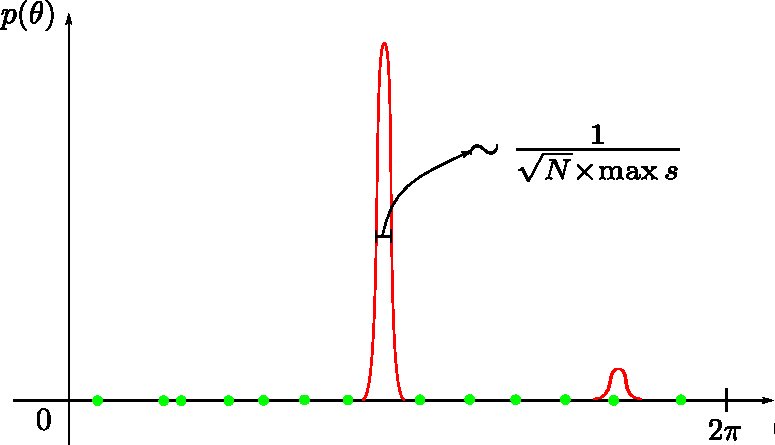
\includegraphics[width=0.45\textwidth]{immagini/numParticles.pdf}
	\end{center}
	\caption{In this example the selected points are too sparse and do not sample correctly the posterior probability distribution.}
	\label{fig:typicalPeak}
\end{figure}
%
Moreover the width of the other peaks in the distribution seems to be experimentally approximately the same of the central peak. In our simulation we took $k =10$. We also insert a lower bound to the number of particles, set arbitrarily to $n_{part} = 3000$. In summary 
%
\begin{equation}
	n_{part} = \max \lbrace \round{k \sqrt{N} \times \max{s}} , 3000 \rbrace \; .
\end{equation}
%
We stress that such analysis applies to the resampling algorithm that \textbf{do not} change the locations of the particles. Those that do, like the Circular resampling, might not be subject to it.


\subsection{Simulations results}
%
In this section we report the results of the simulations for the three resampling algorithms. All the simulations refer to the estimation of the single angle $\theta = 1 \, \text{rad}$, the number of experiments runs from $N = 10$ to $N = 200$ with step $10$. Each point is the the result of $\nu = 30$ simulation that gave estimations $\hat{\theta}_i$ with $i = 1, 2, \dots, \nu$ as results. We plot the MSE
%
\begin{equation}
	\Delta^2 \hat{\theta} = \frac{1}{\nu} \sum_{i=1}^\nu (\hat{\theta}_i - \theta)^2 \; .
\end{equation}
%
as a function of the number of experiments $N$, that is the number of photons used. The number of particles has been chosen according to the rule presented in section~\ref{sec:numPart}, in all cases the resampling threshold has been set to $0.5$. The circular version of the resampling seems to be particularly affected from the tails of the probability distribution. We see indeed that the estimation fails to reach the desired precision. The other strategies give comparable results. In particular there doesn't seems to be a difference between the strategy with the importance resampling and the strategy with the simplified resampling. \textbf{We conclude therefore that the importance resampling is not needed}.
%
\begin{figure}[!t]
	\begin{center}
		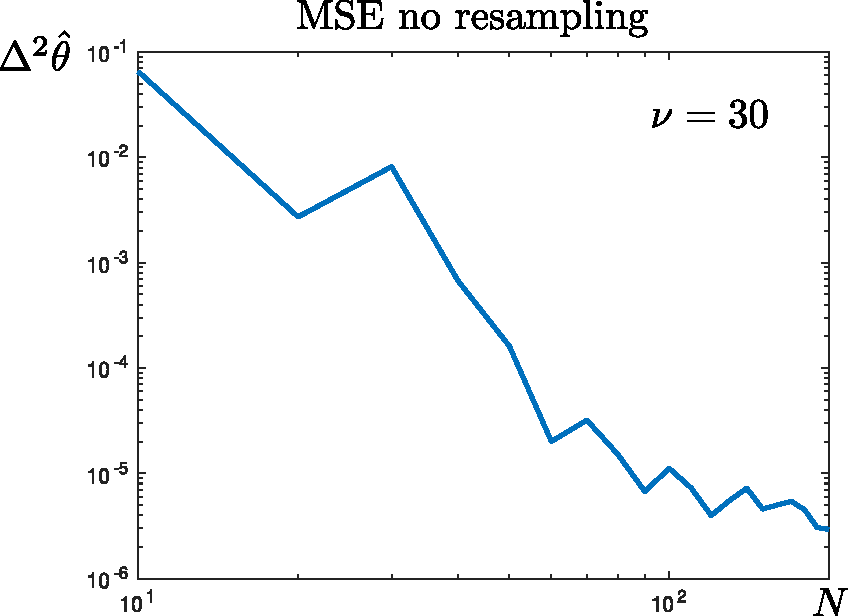
\includegraphics[width=0.45\textwidth]{immagini/noResampling.pdf}
	\end{center}
	\caption{MSE precision for an experiment with no resampling.}
	\label{fig:noResampling}
\end{figure}
%
\begin{figure}[!t]
	\begin{center}
		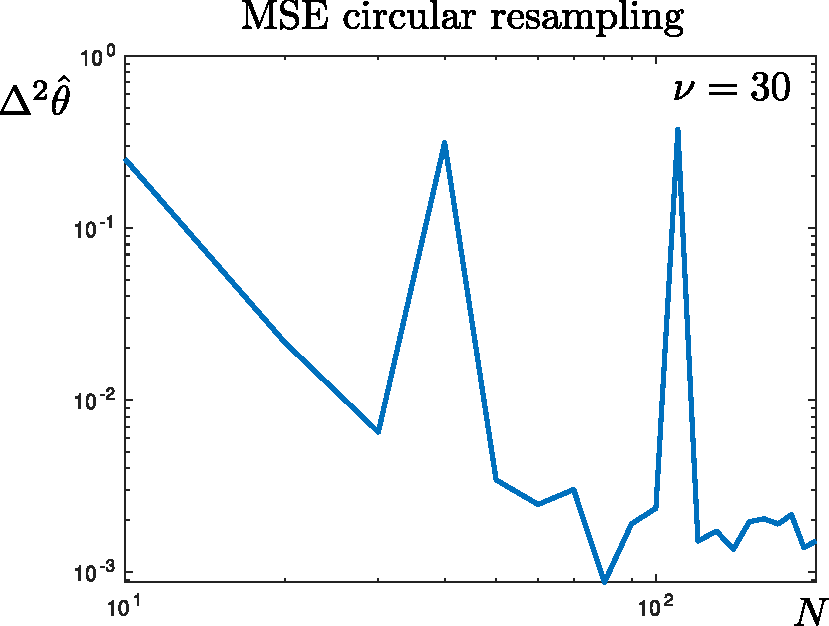
\includegraphics[width=0.45\textwidth]{immagini/circularResampling.pdf}
	\end{center}
	\caption{MSE precision for an experiment with circular resampling, and $a = 0.9$.}
	\label{fig:ircularResampling}
\end{figure}
%
\begin{figure}[!t]
	\begin{center}
		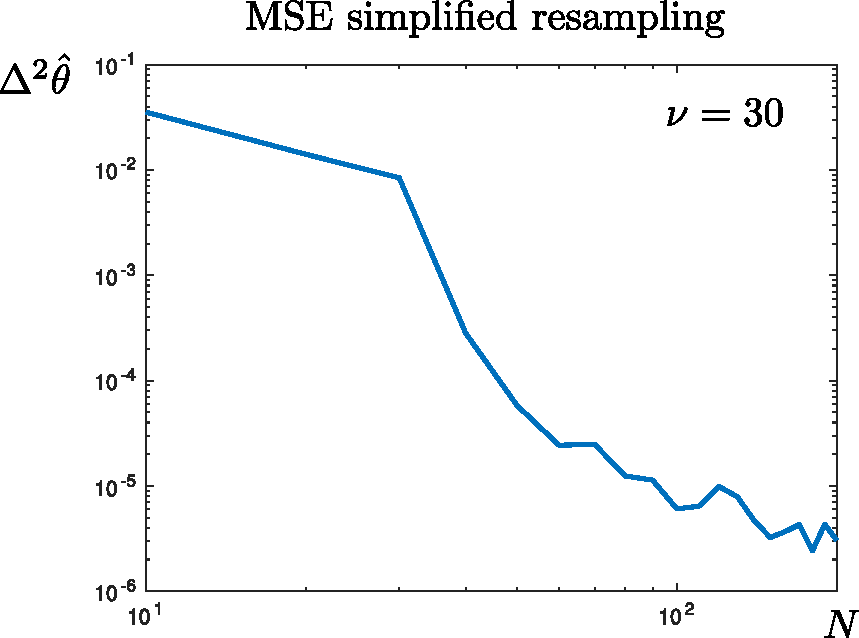
\includegraphics[width=0.45\textwidth]{immagini/simplifiedResampling.pdf}
	\end{center}
	\caption{MSE precision for an experiment with circular resampling, with $a = 0.9$.}
	\label{fig:simplifiedResampling}
\end{figure}
%
\begin{figure}[!t]
	\begin{center}
		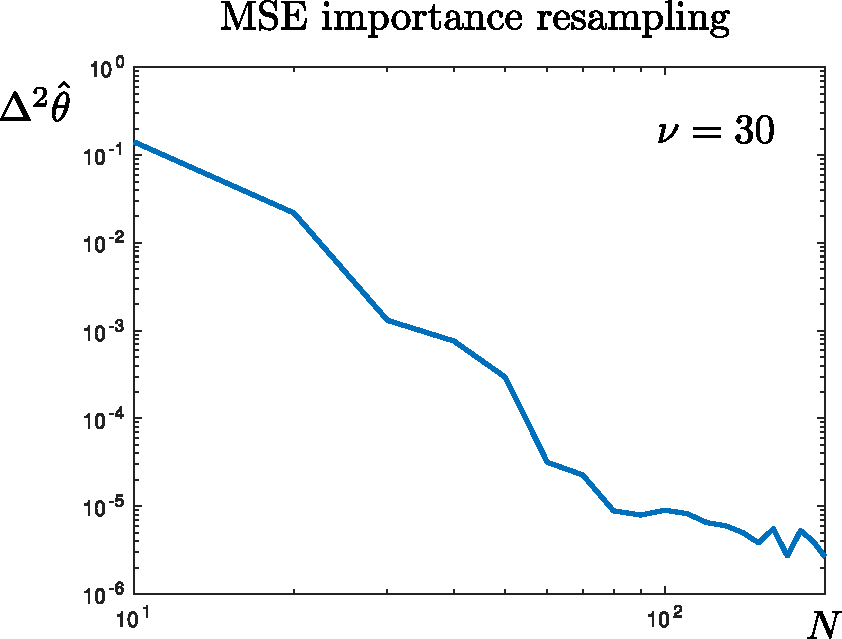
\includegraphics[width=0.45\textwidth]{immagini/importanceResampling.pdf}
	\end{center}
	\caption{MSE precision for an experiment with circular resampling, with $a = 0.9$.}
	\label{fig:importanceResampling}
\end{figure}
%

\section{Errata corrige original paper}
%
There seems to be some minor typos in the source paper~\cite{Granade2012}, that we proceed to list in this section
%
\begin{enumerate}
	
	\item p. 11, the computation of the variance $u_D \leftarrow - \sum_{i} w_i (\boldsymbol{x}_i - \boldsymbol{\mu})^T Q (\boldsymbol{x}_i - \boldsymbol{\mu})$ in Algorithm 5 should contain the updated weights $w_i'$. When estimating a phase this line should be $u_d \leftarrow - \text{estVarianceCircular} (\lbrace \theta_i, w_i' \rbrace)$, as in Algorithm~\ref{alg:utilityNVcircular}.
	
	\item p.12, in Algorithm 7 the resampling condition is $\frac{1}{\sum_{i} w_i^2} \le r \times n_{part}$.
	
\end{enumerate}

\section{Random perturbation}
%
After a resampling procedure with the simplified algorithm or with the importance sampling procedure the diversity of the ensemble is reduced. Because the same positions with high weights is replicated many times. After each resampling we add a Gaussian noise $\mathcal{N} (0, \sigma_p)$ to each particle in order to increase diversity, this procedure is called roughening. Doing so introduces a fundamental limit in the precision of the procedure $\sigma_p$, that should be chosen smaller than the maximum theoretical precision of the Bayesian learning, we chose therefore $\sigma_p = (\sqrt{N} \times \max s)^{-1}$. Some simulation have been performed introducing this noise, but \textbf{no measurable improvement has been observed.}

\section{Sparse considerations}
%
\begin{enumerate}
	
\item A problem that \textbf{might} arise from this settings is that the algorithm requires changing the q-plate for every couple of experiments. Such a thing is definitely not practical when working with a large number of photons, and therefore with a potentially large number of q-plates switches. Whether this is the case or not, must be seen from the simulations. A possible solution to this problem may be to implement regularization of the solution in the utility function, that forces some nice properties of the chosen strategy. This is very similar to what is done in the machine learning field. In our case we want to promote the strategy $c_{N+1}$ equal to $c_{N}$, which could be accomplished via the utility function
%
\begin{equation}
U(c_{N+1}, C; \pi) = -r (\pi, c_{N+1}, C) - \mu \left( 1 - \delta_{C_{N+1}, c_N}\right) \; ,
\end{equation}
% 
where $\delta_{C_{N+1}, c_N} = 1$ if $c_{N+1} = c_N$ and $\delta_{C_{N+1}, c_N} = 0$ if $c_{N+1} \neq c_N$. The parameter $\mu$ controls the strength of this regularization. 

\item How does the optimization of the Bayesian risk performs when the tails of the posterior distribution are important? In particular does the resampling of the ``particles'' remove the contributions of the tails? If this is the case one may consider instead of moving the old particles, just adding new ones where the posterior distribution peaks.
	
\item A first problem that might arise is that the resampling procedure of the particle filter neglects purposely the tails of the distribution. That is, because of their relatively lower weights the tails might not get resampled at all in the algorithm, although they are important for the determination of the variance. This can be corrected via a procedure of importance sampling. Consider an ensemble $\lbrace \theta_i, w_i \rbrace$ produced by the algorithm, instead of sampling directly from it we sample from $\lbrace \theta_i, \tilde{w}_i \rbrace$, where 
%
\begin{equation}
	\tilde{w}_i = f(\theta_i) w_i \; , 
\end{equation}
%
where 
%
\begin{equation}
	f(\theta) = 1 + \frac{1}{\hat{\sigma^2}} (\theta - \hat{\mu})^2 \; ,
\end{equation}
%
where the distance $\theta - \hat{\mu}$ is the angular distance.

	
\textbf{The problem with this approach is that there is no guarantee that $f$ will be centred around the true value. If $\mu$ is particularly off we might enhance the wrong values. This problem is shared by every algorithm that uses dynamical parameters that depend on $\hat{\mu}$ or $\hat{\sigma}$.} 


	
\item A problem that \textbf{might} arise from this settings is that the algorithm requires changing the q-plate for every couple of experiments. Such a thing is definitely not practical when working with a large number of photons, and therefore with a potentially large number of q-plates switches. Whether this is the case or not, must be seen from the simulations. A possible solution to this problem may be to implement regularization of the solution in the utility function, that forces some nice properties of the chosen strategy. This is very similar to what is done in the machine learning field. In our case we want to promote the strategy $c_{N+1}$ equal to $c_{N}$, which could be accomplished via the utility function
%
\begin{equation}
	U(c_{N+1}, C; \pi) = -r (\pi, c_{N+1}, C) - \mu \left( 1 - \delta_{C_{N+1}, c_N}\right) \; ,
\end{equation}
% 
where $\delta_{C_{N+1}, c_N} = 1$ if $c_{N+1} = c_N$ and $\delta_{C_{N+1}, c_N} = 0$ if $c_{N+1} \neq c_N$. The parameter $\mu$ controls the strength of this regularization. 

\item How does the optimization of the Bayesian risk performs when the tails of the posterior distribution are important? In particular does the resampling of the ``particles'' remove the contributions of the tails? If this is the case one may consider instead of moving the old particles, just adding new ones where the posterior distribution peaks.

\item The control $c_i$ may contain also the angle of the final polarization measurement, in order to select it adaptively.

\item We can remove the particles that have weight under a certain cut-off, that could be for example
%
\begin{equation}
	p_{th} = \frac{1}{N \times \max{s} \times n_{part}} \; .
\end{equation}
%

\item Is it really true that under a certain probability the outlier peaks become irrelevant for the computation of the variance? Their frequency seems to be inversely correlated with their size.

\item Maybe it is not the case that the Bayesian method should reproduce the resource distribution of its non-Bayesian counterpart. The method is adaptive and may occasionally produce better results than the Heisenberg scaling. We assume that in the few case that may go wrong the algorithms recognises that and effectively controls the application the q-plates. 


\item We needed to use the circular mean to account for the circular variable.
	
\item There is no stability in the proposed optimal sequence of quantum resources to be used.

\end{enumerate}

\section{Sparse data}
It seems that in the phase estimation problem the resampling step in the particle filter can't be done without a careful analysis. Consider an execution of the algorithm where the resampling procedure resamplingSimplified has been employed, with resampling threshold $r_t= 0.5$, $N=150$, and $n_{part} = 5000$, the output turns out to be

\begin{verbatim}
1: 5
2: 16
11: 16
51: 113
Total number of used resources: 5976
Ratio error/piHS: 1.3964
Ratio error/SQL: 0.056749
---------------------------
cos: 64
sin: 86
---------------------------
Estimator: 1.0021
True Value: 1
\end{verbatim}

Instead when no resampling is made the output is

\begin{verbatim}
1: 13
2: 32
11: 29
51: 76
Total number of used resources: 4272
Ratio error/piHS: 1.7031
Ratio error/SQL: 0.081859
---------------------------
cos: 53
sin: 97
---------------------------
Estimator: 1.0015
True Value: 1
\end{verbatim}

Another example has been computed with $N = 200$ and $n_{part} = 15000$. Without resampling we get

\begin{verbatim}
1: 10
2: 15
11: 47
51: 128
Total number of used resources: 7085
Ratio error/piHS: 2.8584
Ratio error/SQL: 0.10668
---------------------------
cos: 67
sin: 133
---------------------------
Estimator: 0.99731
True Value: 1
\end{verbatim}

With resampling $r_t = 0.5$ we get

\begin{verbatim}
1: 11
2: 13
11: 9
51: 167
Total number of used resources: 8653
Ratio error/piHS: 2.5466
Ratio error/SQL: 0.086007
---------------------------
cos: 168
sin: 32
---------------------------
Estimator: 1.0006
True Value: 1
\end{verbatim}

Another simulation with $n_{part} = 100000$ and no resampling gives

\begin{verbatim}
1: 9
2: 17
11: 38
51: 136
Total number of used resources: 7397
Ratio error/piHS: 2.8622
Ratio error/SQL: 0.10455
---------------------------
cos: 76
sin: 124
---------------------------
Estimator: 1.0009
True Value: 1
\end{verbatim}

which is consistent with the results obtained for $n_{part} = 15000$, showing that more particles aren't needed. The reason of such behaviour is that there are tails in the probability distribution which might contribute greatly to the MSE. Consider
%
\begin{equation}
\Delta^2 \hat{\theta} = \int p(\hat{\theta}) ( \hat{\theta} - \theta)^2 \; d \hat{\theta} \; ,
\end{equation}
%
if there are points in the ensemble $\lbrace \theta_i, w_i \rbrace$ such that $p(\theta_i) \sim \Delta^2 \hat{\theta}$ and $\theta_i - \theta \sim 1$, then this points have a considerable effect on the RMSE, even if due to their low probability $p(\theta_i) \sim \frac{1}{N \times (\max{s})^2}$ they won't be resampled. Not even with $n_{part} \sim \sqrt{N} \times \max{s}$. We now try the function resamplingCircular, which implements a mixture of the resampled data with a Gaussian extraction. With $N = 200$ and $n_{part} = 15000$ we get

\begin{verbatim}
1: 5
2: 24
11: 151
51: 20
Total number of used resources: 2734
Ratio error/piHS: 20.8146
Ratio error/SQL: 1.2506
---------------------------
cos: 153
sin: 47
---------------------------
Estimator: 0.98579
True Value: 1
\end{verbatim}

Clearly the estimation is not working.

\section{Talk with Hoch}

\begin{itemize}
	\item In a first version of the algorithm we consider only the possibility of choosing between two phases $0$ and $\frac{\pi}{2}$. A second version may consider a continuous choice of the polarization to measure, but only in the form $\frac{1}{\sqrt{1+\alpha^2}} \left( \ket{0} + \alpha \ket{1} \right)$, with $\alpha \in \mathbb{R}$. A more evolved version of the experiment could account for complex values of $\alpha$, by using two lamina.
	 
	\item Hoch points toward a possible problem. Weighting all the particles uniformly after performing an update may be a too rough way of dealing with the weights update.
	
	\item Hoch says that taking $n_{part} =  \max{s} \times N \times 10$ might be too much. In particular he says such a number of particles may apply in the case no resampling is made, but is not optimal when the resampling is activated. In that case we should choose the number of particles to be $\max{s} \times 100$ if we want $100$ particle in each peak of the probability distribution.
	
	\item Francesco proposes an alternative way to approximate the probability distribution that is the use of the {\textbf{Varanoi cells}}. According to that we should abandon the approximation of the posterior distribution with a series of point, in favour of a distribution in terms of a series of cell. But because the algorithm seems to work well without this add-on, therefore is doesn't seems necessary at the moment to go down this road.
	
	\item The resampling condition is $\frac{1}{\sum_{i} w_i^2} \le r \times n_{part}$.
	
	\item The reduced particle approximation is used only to pass an input to the utility function. It means in no way that the number of particles should be reduced during the algorithm execution. That would maybe give the correct final result for the estimation but 
	
	\item \textbf{Idea}: I could try to implement a Bayesian filter that would work for a multimodal distribution. Or I could consider the potential given by the probability distribution and move the particles according to the potential, with the Newton's law. This has the disadvantage of moving very slowly the  particles that are in a plateau of the potential (are are potentially useless there). In any way what should be built is a filter, that identifies the position of the \textbf{local maxima} and tries to concentrate the particles in the maxima.
	%
	\begin{figure}[!t]
		\begin{center}
			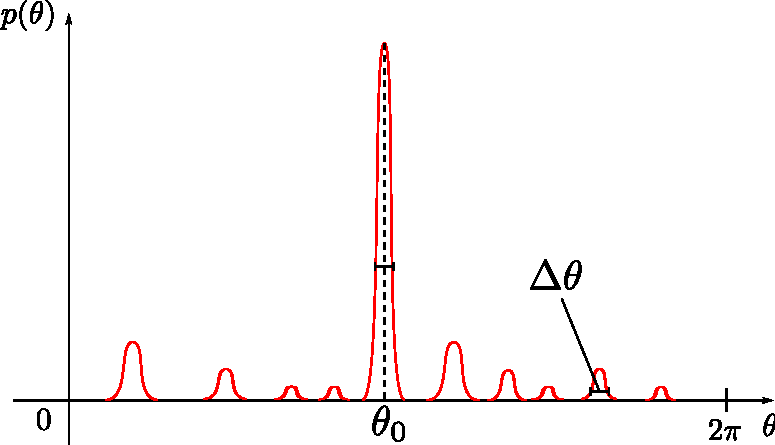
\includegraphics[width=0.45\textwidth]{immagini/typical.pdf}
		\end{center}
		\caption{Typical form of a posterior probability distribution. The secondary peaks are significantly lower that the principal one. A multimodal resampling technique may be able to capture properties of the distributions.}
		\label{fig:typical}
	\end{figure}
	%
	\item Another idea that might help accounting for the tails in the \textbf{importance sampling}. That is, each time we need to resample, instead of extracting the new particle locations from the probability distribution for $\theta$, we extract it from $f(\theta) p(\theta)$ which somehow overweights the tails. It is worth taking a look into the \textbf{multi-modal Gaussian filtering} literature.
	  
	\item Hoch says that there is no real problem in the resampling process. The HS starts after $100$ experiments.
	
	\item Maybe taking the logarithm of the probability distribution and sampling according to the logarithm would produce a more reliable particle distribution.
	
	\item I might try to order the particles according to their contribution to the variance in the computation of the utility function. I might sample the particles according to their probability but according to the impact they have on the variance.
	
	\item In the usual resampling procedure (not with the added Gaussian) sampling from the original distribution with repetitions will work if the particle number is sufficiently large. In particular it should be $N_{part} \gg \max{s} \times N$. So that no points with a significant contribution to the variance is not sampled. E.g.: a certain region with composite probability $10^{-3}$ is unlikely to be sampled with $100$ particles. Therefore we are loosing a contribution of $10^{-3}$ to the variance. Which might although be fundamental if we are doing $N = 1000$ experiments. Therefore the time to perform this algorithm scales quadratically in $N$. I want to find a better scaling, by using less particles.
	
	\item Neglecting the tail of the distribution will inevitably cause errors. As an example compare the following two debug example collected respectively for a simulation with resample threshold $r_t = 0.5$ and $r_t = 0$, both having $n_{part} = 100000$, and $N = 200$ experiments.
	
	
	\begin{verbatim}
	Without resampling:
	
	1: 8
	2: 10
	4: 7
	8: 4
	16: 9
	32: 3
	64: 159
	Total number of used resources: 10504
	Ratio error/piHS: 7.3955
	Ratio error/SQL: 0.22669
	---------------------------
	cos: 168
	sin: 32
	---------------------------
	Estimator: 1.0022
	True Value: 1
	
	N = 50 
	
	1: 7
	2: 5
	4: 5
	8: 3
	16: 4
	32: 3
	64: 23
	Total number of used resources: 1693
	Ratio error/piHS: 1.2744
	Ratio error/SQL: 0.097303
	---------------------------
	cos: 29
	sin: 21
	---------------------------
	Estimator: 1.0024
	True Value: 1
		
	\end{verbatim}
	
	\begin{verbatim}
	With resampling:
	
	1: 6
	2: 4
	4: 6
	8: 6
	16: 4
	32: 4
	64: 170
	Total number of used resources: 11158
	Ratio error/piHS: 4.399
	Ratio error/SQL: 0.13083
	---------------------------
	cos: 101
	sin: 99
	---------------------------
	Estimator: 1.0012
	True Value: 1
	
	N = 50 
	
	1: 8
	2: 5
	4: 5
	8: 4
	16: 3
	32: 4
	64: 21
	Total number of used resources: 1590
	Ratio error/piHS: 1.9171
	Ratio error/SQL: 0.15105
	---------------------------
	cos: 16
	sin: 34
	---------------------------
	Estimator: 0.99621
	True Value: 1
		
	\end{verbatim}
	
	The resampling algorithm was the simplified one: extraction with repetition from the particle ensemble.
	
	\item In order to sample correctly the tails of the distribution we could multiply it with the weight function
	%
	\begin{equation}
		f(\theta) = 1 + \frac{1}{\hat{\sigma^2}} (\theta - \hat{\mu})^2 \; .
	\end{equation}
	%
	The distance $\theta - \hat{\mu}$ is the angular distance. In the following we give an example of a simulation with $N = 35$, $n_ {part} = 5000$ with the importance resampling active, mounted upon a simplified resampling.
	
	\begin{verbatim}
	>> bayesianEstimator
	1: 13
	2: 4
	4: 5
	8: 3
	16: 3
	32: 3
	64: 4
	Total number of used resources: 465
	Ratio error/piHS: 0.078688
	Ratio error/SQL: 0.011464
	---------------------------
	cos: 15
	sin: 20
	---------------------------
	Estimator: 0.99947
	True Value: 1
	\end{verbatim}
	
	If we use the the simplified resampling only, without the importance resampling we get
	
	\begin{verbatim}
	1: 4
	2: 3
	4: 2
	8: 3
	16: 3
	32: 4
	64: 16
	Total number of used resources: 1242
	Ratio error/piHS: 1.0532
	Ratio error/SQL: 0.093886
	---------------------------
	cos: 16
	sin: 19
	---------------------------
	Estimator: 1.0027
	True Value: 1
	\end{verbatim}
	
	Not using the importance sampling means neglecting the tails of the distribution and therefore underestimating the amount of low quantum number states to be used. A resampling procedure is said to be \textbf{unbiased} when $\mathbb{E} \left[N_i'\right] = N w_i$. The expectation values of the number of times the $i$-th particle is extracted is consistent with the weight. This is not true in our case but the unbiasedness is corrected at the level of weights.
	
	\item We also need to introduce a resampling algorithm that will respect the multi-modal nature of the system.

	\item Another method that could be used to sample efficiently the tails is to divide the particles in two groups: one with high weights and one with low weights. The first group, called group A, has a compound probability $1-f = \sum_{a \in A} w_{i}$, while group B has $f = \sum_{a \in B} w_{i}$. W sample independently from this two groups and then weigh the particles in group A with $w_i' = \frac{1-f}{N_A}$ and group $B$ with $w_i' = \frac{f}{N_B}$. \textbf{This technique has not been considered because of the arbitrary of the choice of $f$}. 
	
	\item To increase the diversity of the sample while keeping the number of particles constant one may sample from a smoothed distribution instead of the original one. Define $p(\theta) = \sum_{i=1}^{n_{part}} w_i \delta \left(\theta - \theta_i \right)$ as the discretized approximation. Then we can take the convolution of such distribution with a Gaussian 
	%
	\begin{equation}
		g(t) = \frac{1}{\sqrt{2 \pi} \sigma_p} \exp \left( -\frac{1}{2} \frac{t^2}{\sigma_p^2} \right) \; ,
	\end{equation}
	%
	where $\sigma_p$ is the precision associated to the smoothing process. It should be $\sigma_p \simeq k \hat{\sigma}$, this precision should be chosen in order to not lose the importat features of the probability distribution. We build a continuous probability distribution by convolving $p(\theta)$ with $g(t)$, that is
	%
	\begin{eqnarray}
		p_{cont} (\theta) &=& \int_{-\infty}^{+\infty} f(\theta-t) g(t) d t \\ &=& \sum_{i=1}^{n_{part}} w_i \, g(\theta - \theta_i) \; .
	\end{eqnarray}
	%
	
	 Now we generate randomically an element $\theta_{r}$ uniformly in $\left[0, 2 \pi \right]$ and accept each generated angle if and only if $r \ge p_{cont} (\theta_r)$, where $r$ is randomly generated number in $\left[0, 1 \right]$. Notice that the computational cost of performing the convolution doesn't depend on the precision of the convolution. This procedure works but might have an enormous computational cost if the distribution is very concentrated. We propose therefore the following alternative. The original dataset $\lbrace w_i, \theta_i \rbrace$ is substituted with the convoluted dataset $\lbrace \tilde{w}_i, \theta_i \rbrace$, where $\tilde{w}_i = p_{cont} (\theta_i)$. Then we should resample $\lbrace \tilde{w}_i, \theta_i \rbrace$ but substitute any new $\theta_i'$ with a perturbed version $\theta_i' + \delta$ where $\delta \sim g$ is a Gaussian noise. We set the weight of $\theta_i'$ using  $p_{cont} (\theta_i'+\delta)$. It is not clear that this can be done while conserving the goodness of the obtained example, .i.e. that it correctly represents the probability distribution.
	 
	 It is clear that if we want to introduce a some new particles we need an estimator for the probability distribution in between the given particles. This can be obtained via a linear interpolation or via a convolution.
	 
	 \item Maybe the very simple approach of \textbf{roughening} the distribution at each resampling with a noise $N(0, \sigma_p)$ with $\sigma_p \simeq \frac{1}{\sqrt{N} \times \max{s}}$ at each resampling, while keeping the same weight as the original unperturbed particle. Introducing such a phenomenon means limiting the precision of the particle filter, but if we choose a $\sigma_p$ that is anyway smaller than the theoretical precision of the filter (which cannot beat the HS), then the perturbation should be small, while we are gaining diversity in the particle locations.
	 
	 We could also apply the roughening procedure to all particles at each experiment.
	 
	 The width of central peak in the probability distribution is limited by the Heisenberg scaling, because even if the neglect the contributions of the tails there is the shoot noise of the last stage with $\max{s}$ as quantum resource, which means that the central peak cannot be smaller than $\frac{1}{\max{s} \times \sqrt{N}}$.
	 
	 \item Another viable route is to start with a large number of particles able to represent the finer details of the probability distribution and eliminate the particles sampled multiple times, by accumulating all their weight on a single particle.
	 
	 \item Maybe in order to solve the tail problem it is just sufficient to resample less (or not to resample).	 
	
\end{itemize}

\section{Talk with Valeria ed Emanuele 4/10/21}

\begin{itemize}
	
	\item Valeria says that the new experiment with the sequential Montecarlo must be compared to a version of the old phase estimation algorithm (mine). It could be done by introducing stochastic visibilities that are (stochastically) generated for an instance of the experiment and are stochastically learned by the sequential Montecarlo approach, while my algorithm only knows an approximate value for the visibilities.
	
	\item Can we use the reinforcement learning in this kind of problem? Can the q-plate that we must use be decided via reinforcement learning?
	
	\item I should study the visibilities as nuisance parameters. They can't anyway be measured with HS precision.
	
\end{itemize}


%\section{Bayesian estimation with unknown visibilities}
%
%In the following we report the results for a Bayesian estimation we have done, where we kept the visibilities unknown (and equal to $V = 0.90$ for all the steps). The error we plot is only that of the phase but the decision process of the algorithm was run with $Q = \id$. The simplified resampling strategy is arguably the one that performs better. The importance resampling doesn't seem to work. If anything it seems not to work. The performances of the circular resampling are comparable to that of the no resampling case.
%
%\begin{figure}[!t]
%	\begin{center}
%		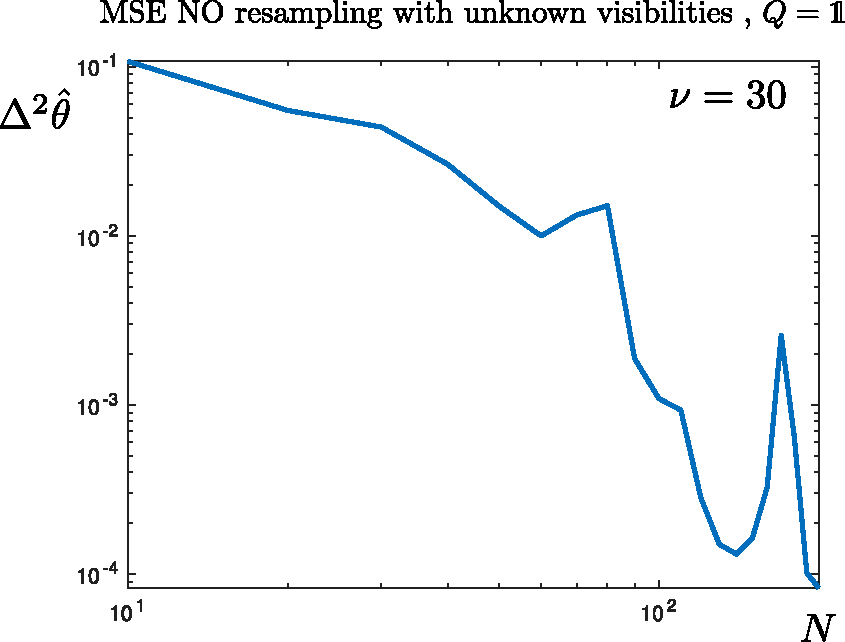
\includegraphics[width=0.45\textwidth]{immagini/simplifiedNoResamplingVisibilitiesQIdentity.pdf}
%	\end{center}
%	\caption{MSE precision for a Bayesian estimation procedure without resampling and with unknown visibilities (set to $V = 0.90$). Each experiment has been repeated $\nu = 30$ times and the unknown phase was $\theta = 1$.}
%	\label{fig:simplifiedNoResamplingVisibilitiesQIdentity}
%\end{figure}
%
%\begin{figure}[!t]
%	\begin{center}
%		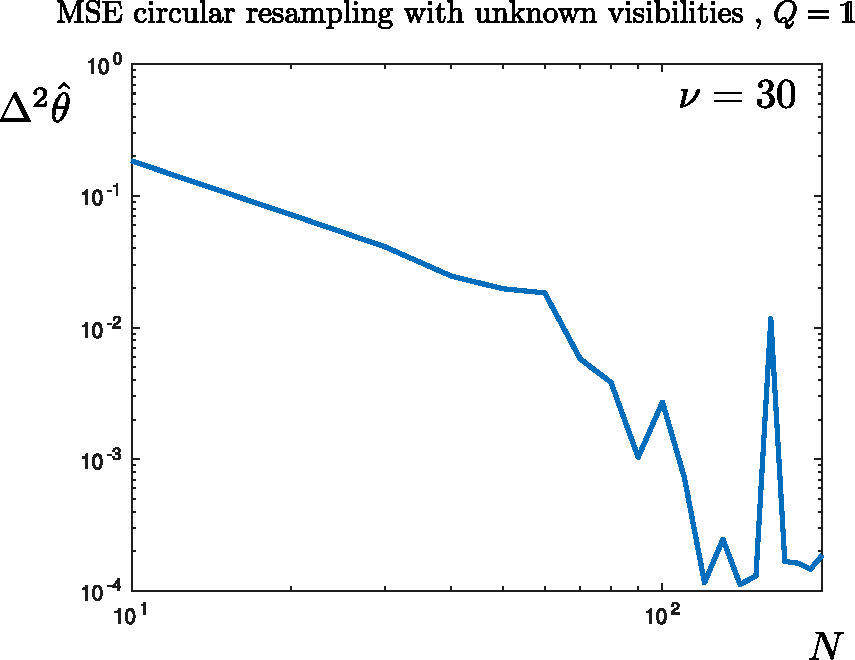
\includegraphics[width=0.45\textwidth]{immagini/circularResamplingVisibilitiesQIdentity.pdf}
%	\end{center}
%	\caption{MSE precision for a Bayesian estimation procedure with circular resampling and with unknown visibilities (set to $V = 0.90$). Each experiment has been repeated $\nu = 30$ times and the unknown phase was $\theta = 1$.}
%	\label{fig:circularResamplingVisibilitiesQIdentity}
%\end{figure}
%
%\begin{figure}[!t]
%	\begin{center}
%		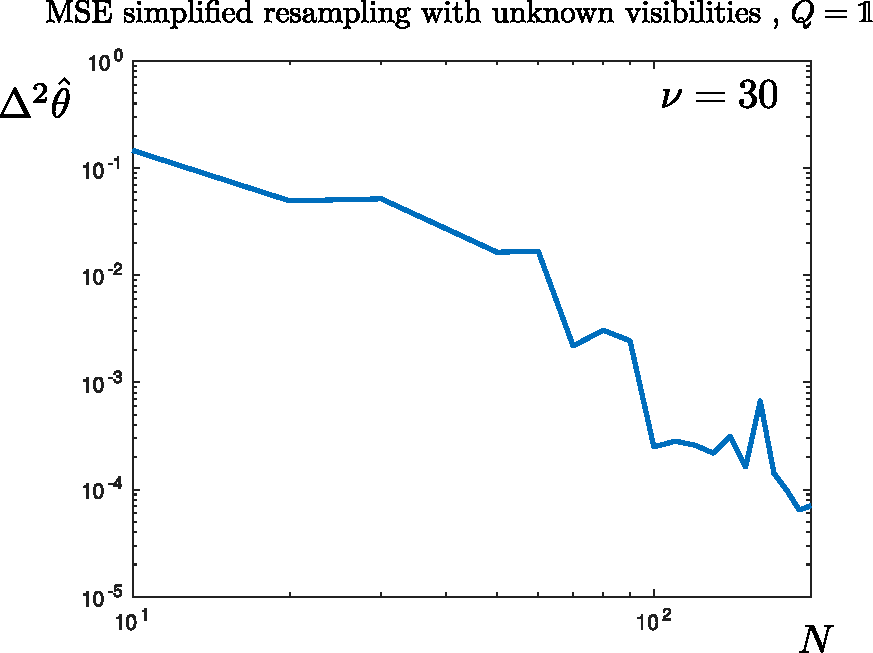
\includegraphics[width=0.45\textwidth]{immagini/simplifiedResamplingVisibilitiesQIdentity.pdf}
%	\end{center}
%	\caption{MSE precision for a Bayesian estimation procedure with simplified resampling and with unknown visibilities (set to $V = 0.90$). Each experiment has been repeated $\nu = 30$ times and the unknown phase was $\theta = 1$.}
%	\label{fig:simplifiedResamplingVisibilitiesQIdentity}
%\end{figure}
%
%\begin{figure}[!t]
%	\begin{center}
%		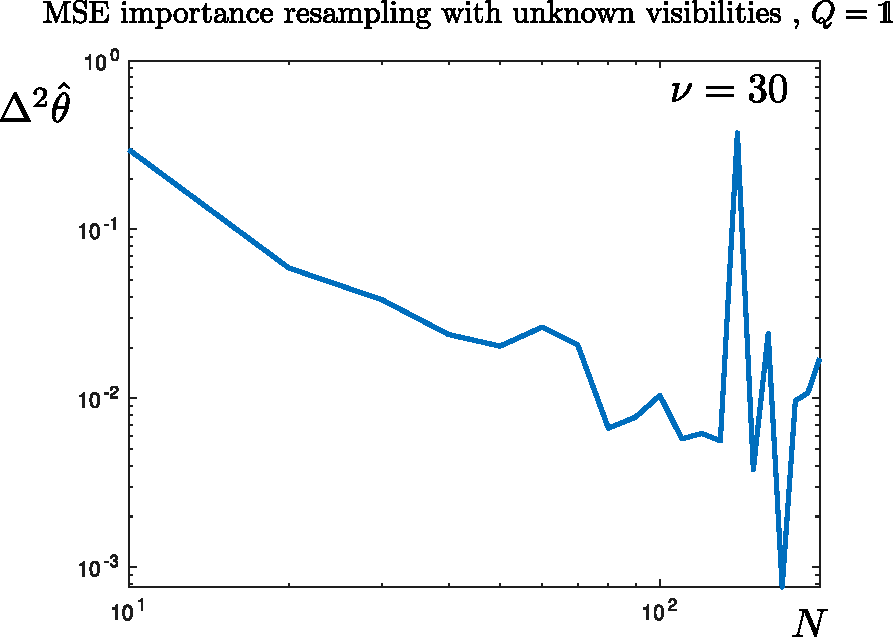
\includegraphics[width=0.45\textwidth]{immagini/importanceResamplingVisibilitiesQIdentity.pdf}
%	\end{center}
%	\caption{MSE precision for a Bayesian estimation procedure with simplified importance resampling and with unknown visibilities (set to $V = 0.90$). Each experiment has been repeated $\nu = 30$ times and the unknown phase was $\theta = 1$.}
%	\label{fig:importanceResamplingVisibilitiesQIdentity}
%\end{figure}

%\section{Limited number of particles}
%
%The real hurdle in performing Bayesian phase estimation is the number of required particles. In this section we report some simulations performed with the fixed number of particles $n_{part} = 1000$, and we compared the circular resampling strategy to an importance resampling strategy in which diversity has been promoted with a roughening procedure. 
%
%\begin{figure}[!t]
%	\begin{center}
%		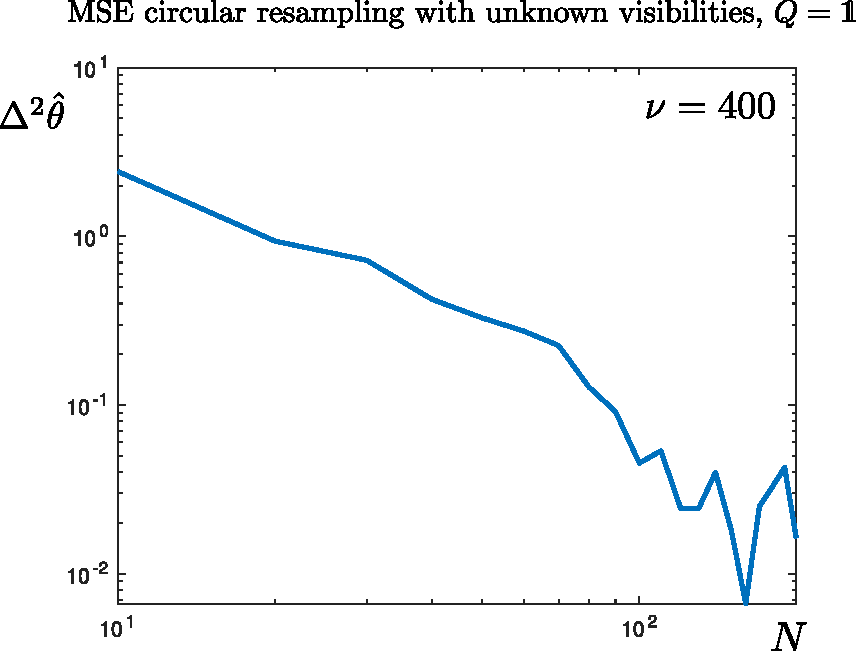
\includegraphics[width=0.45\textwidth]{immagini/circularEstimationwith400experiments.pdf}
%	\end{center}
%	\caption{MSE precision for a Bayesian estimation procedure with circular resampling and with unknown visibilities (set to $V = 0.90$). Each experiment has been repeated $\nu = 400$ times and the unknown phase was $\theta = 1$.}
%	\label{fig:circularEstimationwith400experiments}
%\end{figure}
%
%\begin{figure}[!t]
%	\begin{center}
%		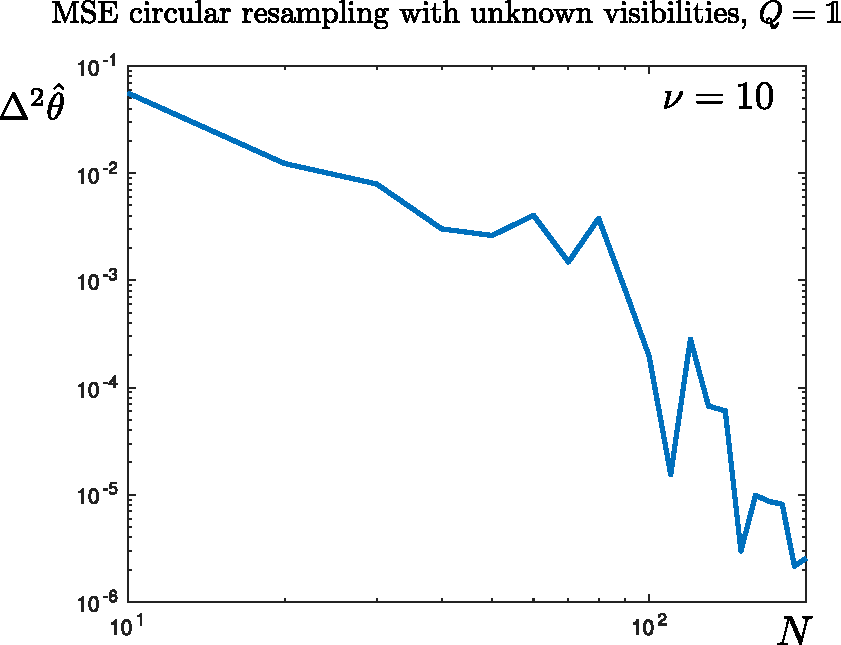
\includegraphics[width=0.45\textwidth]{immagini/circularEstimationwith10experiments.pdf}
%	\end{center}
%	\caption{MSE precision for a Bayesian estimation procedure with circular resampling and with unknown visibilities (set to $V = 0.90$). Each experiment has been repeated $\nu = 10$ times and the unknown phase was $\theta = 1$.}
%	\label{fig:circularEstimationwith10experiments}
%\end{figure}
%
%\begin{figure}[!t]
%	\begin{center}
%		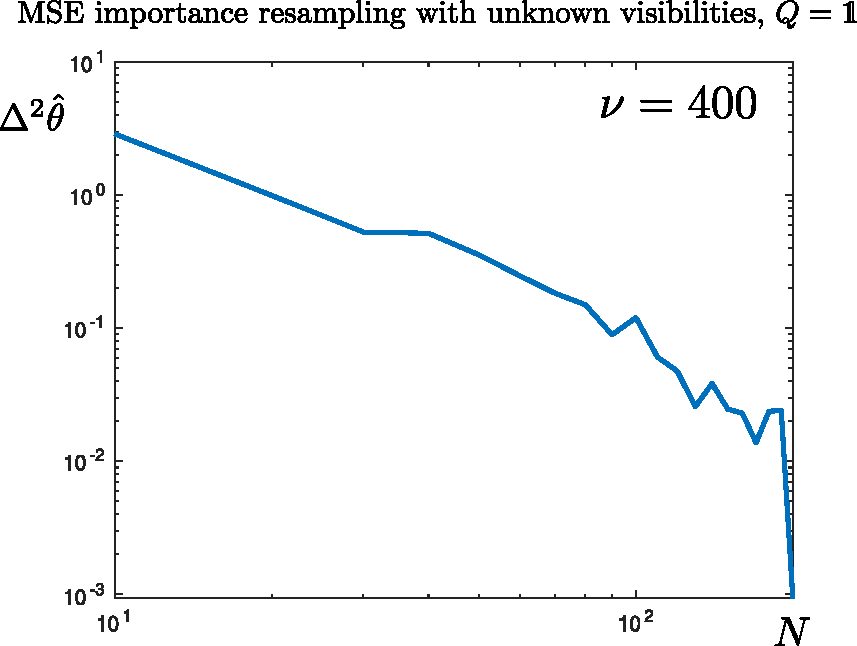
\includegraphics[width=0.45\textwidth]{immagini/importanceResamplingWithRandomization400experiments.pdf}
%	\end{center}
%	\caption{MSE precision for a Bayesian estimation procedure with simplified importance resampling and with unknown visibilities (set to $V = 0.90$). Each experiment has been repeated $\nu = 400$ times and the unknown phase was $\theta = 1$. A roughening procedure has been performed after each resampling.}
%	\label{fig:importanceResamplingWithRandomization400experiments}
%\end{figure}
%
%\begin{figure}[!t]
%	\begin{center}
%		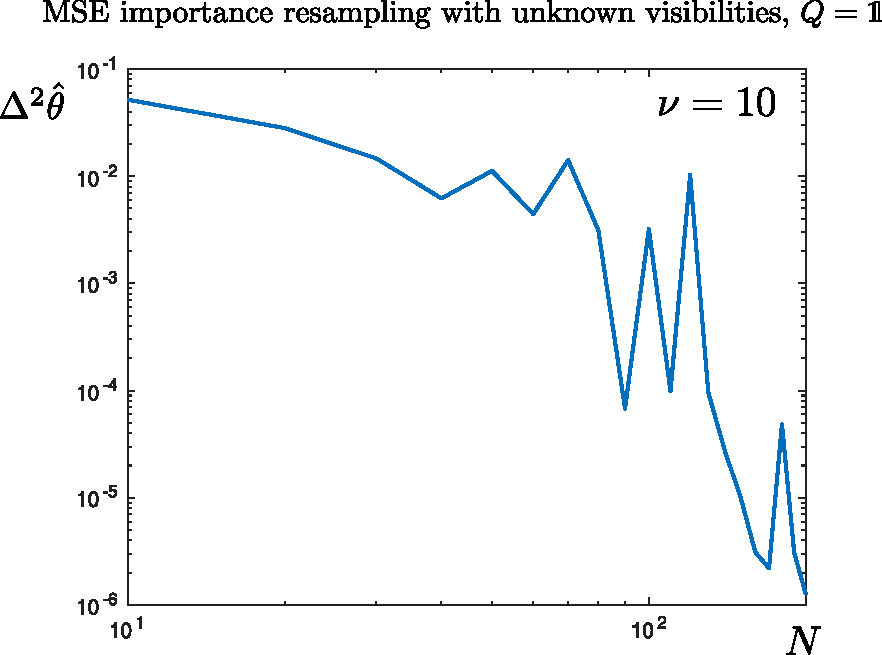
\includegraphics[width=0.45\textwidth]{immagini/importanceResamplingwith10experiments.pdf}
%	\end{center}
%	\caption{MSE precision for a Bayesian estimation procedure with simplified importance resampling and with unknown visibilities (set to $V = 0.90$). Each experiment has been repeated $\nu = 10$ times and the unknown phase was $\theta = 1$. A roughening procedure has been performed after each resampling.}
%	\label{fig:importanceResamplingwith10experiments}
%\end{figure}
%
%It is clear that a small number of particles cannot reproduce the Heisenberg scaling, this is due to the high probability terms of the phase distribution. \textbf{We wonder whether it is possible at all to reach Heisenberg scaling with a small number of particles. This plots are wrong because I made an error in the plot stage. It seems that the tail problem is only marginally a problem of the phase estimation process.}


\appendix

\section{Form of the $f(\theta)$ function}
%
First of all let us indicate with $\theta_0$ the true value of the phase and with $\Delta \hat{\theta}$ the RMSE error $\Delta \hat{\theta} := \sqrt{\Delta^2 \hat{\theta}}$. A typical posterior probability distribution for the angle $\theta$ look like in Fig.~\ref{fig:typicalModified}. We have a central peak in the position of the true value $\theta_0$ and many scattered secondary peaks. Our objective is to find a function that enhances the secondary peaks and brings them to the level of the principal one.
%
\begin{figure}[!t]
	\begin{center}
		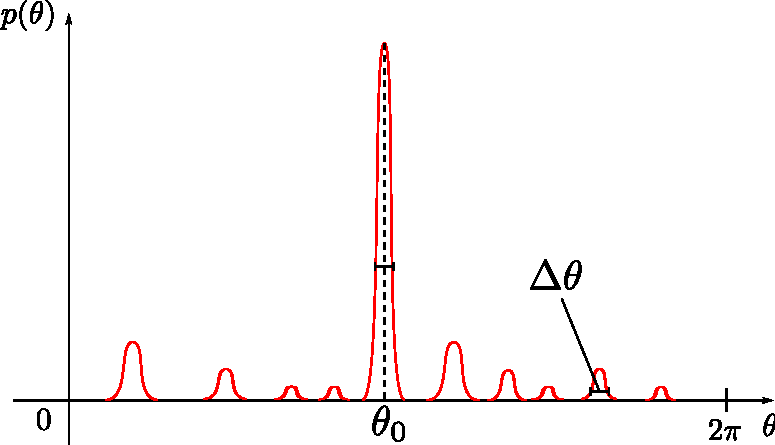
\includegraphics[width=0.45\textwidth]{immagini/typical.pdf}
	\end{center}
	\caption{Typical form of a posterior probability distribution. The secondary peaks are significantly lower that the principal one.}
	\label{fig:typicalModified}
\end{figure}
%
The form of the function $f(\theta)$ comes from an heuristic arguments that we discuss in this section. Experimentally we observe that the secondary peaks have size $\Delta \theta \simeq \Delta \hat{\theta}$, which is small for $N \gg 1$, so that we can consider the peak localized at its position $\theta$. Therefore its contribution to the MSE is
%
\begin{equation}
	\int p(\hat{\theta}) (\hat{\theta}-\theta_0)^2 d \hat{\theta} \sim \bar{p}(\theta) (\theta-\theta_0)^2 \Delta \hat{\theta} \; .
\end{equation}
% 
where $\bar{p}(\theta)$ is the characteristic probability of the peak. Such contribution must be relevant when compared to the MSE $\Delta^2 \hat{\theta}$:
%
\begin{equation}
	\bar{p}(\theta) (\theta-\theta_0)^2 \Delta \hat{\theta} \sim \Delta^2 \hat{\theta} \; ,
\end{equation}
%
that means those peaks with probability density 
%
\begin{equation}
	\bar{p}(\theta) \simeq \frac{\Delta \hat{\theta}}{(\theta-\theta_0)^2} \; .
\end{equation}
%
will contribute to the MSE. The function $f(\theta)$ is chosen to make the probability $\bar{p} (\theta) \Delta \hat{\theta}$ of sampling from the peak of order $\mathcal{O}(1)$, that is
%
\begin{equation}
	f(\theta) \hat{p} (\theta) \Delta \hat{\theta} \sim f(\theta) \frac{\Delta^2 \hat{\theta}}{(\theta-\theta_0)^2} \sim 1 \; . 
\end{equation}
%
Therefore on the secondary peaks the function $f(\theta)$ should have value $\sim \frac{(\theta-\theta_0)^2}{\Delta^2 \hat{\theta}}$, while near the principal one it should be $f(\theta) \sim 1$. We choose
%
\begin{equation}
	f(\theta) = 1 + \frac{(\theta-\theta_0)^2}{\Delta^2 \hat{\theta}} \; ,
\end{equation}
%
as an interpolating approximation. Of course the true MSE and $\theta_0$ are unknown during the execution and we should use the approximate values $\hat{\mu}$ and $\hat{\sigma}$. Notice that the algorithm will perform a correct resampling for whatever reasonable function $f(\theta)$, it is a matter of choosing a convenient one. 



\begin{thebibliography}{100}
	
\bibitem{Granade2012} C E Granade et al 2012 \href{https://doi.org/10.1088/1367-2630/14/10/103013}{New J. Phys. {\bf 14} 103013}

\bibitem{Hol2006} J D Hol, T B Schon, and F Gustafsson 2006 \href{http://ieeexplore.ieee.org/document/4378824/}{2006 IEEE Nonlinear Statistical Signal Processing Workshop}

\bibitem{Li2015} T Li, M Bolic, and P M Djuric 2015 \href{https://ieeexplore.ieee.org/document/7079001/}{IEEE Signal Process. Mag. {\bf 32} 70-86}
	
\end{thebibliography}

\end{document}